% Component Diagram cho GraphRAG QA Pipeline
% Sử dụng trong LaTeX với % Component Diagram cho GraphRAG QA Pipeline
% Sử dụng trong LaTeX với % Component Diagram cho GraphRAG QA Pipeline
% Sử dụng trong LaTeX với % Component Diagram cho GraphRAG QA Pipeline
% Sử dụng trong LaTeX với \input{architecture_graphrag_diagram.tex}

\begin{figure}[H]
\centering
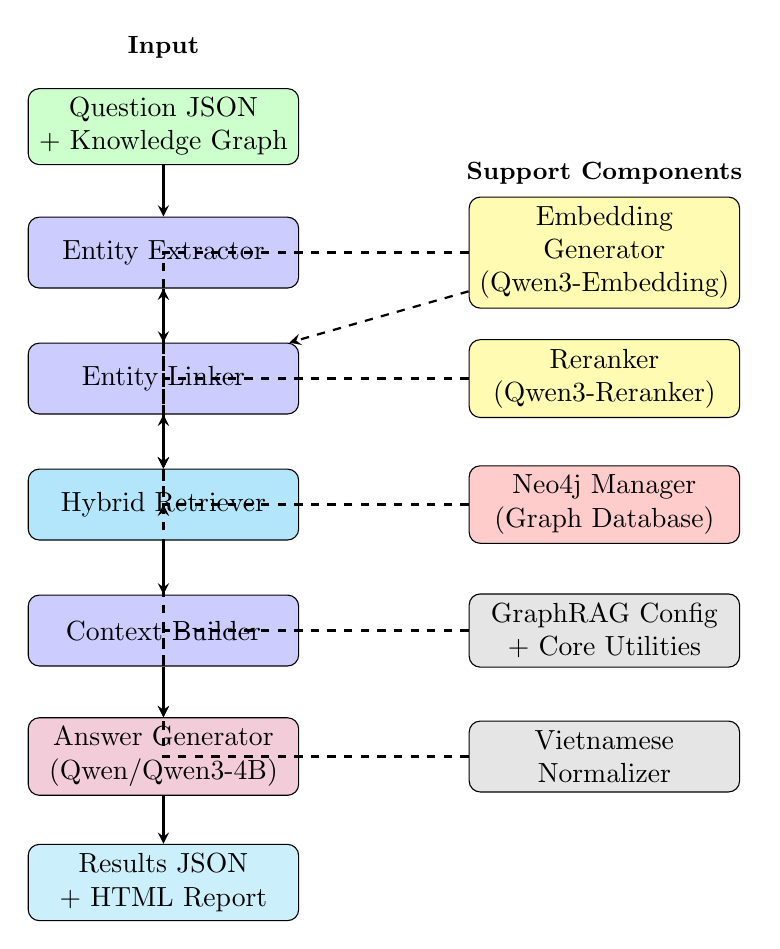
\begin{tikzpicture}[node distance=1.6cm, auto]
    % Styles
    \tikzstyle{datablock} = [rectangle, draw, fill=green!20, 
        text width=3.2cm, text centered, rounded corners, minimum height=0.9cm]
    \tikzstyle{component} = [rectangle, draw, fill=blue!20, 
        text width=3.2cm, text centered, rounded corners, minimum height=0.9cm]
    \tikzstyle{apiblock} = [rectangle, draw, fill=orange!20, 
        text width=3.2cm, text centered, rounded corners, minimum height=0.9cm]
    \tikzstyle{dbblock} = [rectangle, draw, fill=red!20, 
        text width=3.2cm, text centered, rounded corners, minimum height=0.9cm]
    \tikzstyle{modelblock} = [rectangle, draw, fill=purple!20, 
        text width=3.2cm, text centered, rounded corners, minimum height=0.9cm]
    \tikzstyle{outputblock} = [rectangle, draw, fill=cyan!20, 
        text width=3.2cm, text centered, rounded corners, minimum height=0.9cm]
    \tikzstyle{arrow} = [thick,->,>=stealth]
    \tikzstyle{dashedarrow} = [thick,->,>=stealth,dashed]
    
    % === LEFT COLUMN: Main Pipeline ===
    % Input
    \node [datablock] (input) {Question JSON\\+ Knowledge Graph};
    
    % Entity Extractor
    \node [component, below of=input] (entityext) {Entity Extractor};
    
    % Entity Linker
    \node [component, below of=entityext] (entitylink) {Entity Linker};
    
    % Hybrid Retriever
    \node [component, below of=entitylink, fill=cyan!30] (retriever) {Hybrid Retriever};
    
    % Context Builder
    \node [component, below of=retriever] (ctxbuilder) {Context Builder};
    
    % Answer Generator
    \node [modelblock, below of=ctxbuilder] (answergen) {Answer Generator\\(Qwen/Qwen3-4B)};
    
    % Output
    \node [outputblock, below of=answergen] (output) {Results JSON\\+ HTML Report};
    
    % === RIGHT COLUMN: Components ===
    % Embedding Generator
    \node [component, right of=entityext, xshift=4cm, fill=yellow!30] (embedding) {Embedding Generator\\(Qwen3-Embedding)};
    
    % Reranker
    \node [component, below of=embedding, fill=yellow!30] (reranker) {Reranker\\(Qwen3-Reranker)};
    
    % Neo4j Manager
    \node [dbblock, below of=reranker] (neo4j) {Neo4j Manager\\(Graph Database)};
    
    % Core/Config
    \node [datablock, below of=neo4j, fill=gray!20] (config) {GraphRAG Config\\+ Core Utilities};
    
    % Vietnamese Normalizer
    \node [datablock, below of=config, fill=gray!20] (normalizer) {Vietnamese\\Normalizer};
    
    % === ARROWS: Main Flow ===
    \draw [arrow] (input) -- (entityext);
    \draw [arrow] (entityext) -- (entitylink);
    \draw [arrow] (entitylink) -- (retriever);
    \draw [arrow] (retriever) -- (ctxbuilder);
    \draw [arrow] (ctxbuilder) -- (answergen);
    \draw [arrow] (answergen) -- (output);
    
    % === ARROWS: Dependencies ===
    \draw [dashedarrow] (embedding) -- (entitylink);
    \draw [dashedarrow] (embedding) -| (retriever);
    \draw [dashedarrow] (reranker) -| (retriever);
    \draw [dashedarrow] (neo4j) -| (retriever);
    \draw [dashedarrow] (neo4j) -| (entitylink);
    \draw [dashedarrow] (config) -| (answergen);
    \draw [dashedarrow] (normalizer) -| (entityext);
    
    % === Labels ===
    \node [above of=input, yshift=-0.6cm, font=\small\bfseries] {Input};
    \node [above of=embedding, yshift=-0.6cm, font=\small\bfseries] {Support Components};
    
\end{tikzpicture}
\caption{Kiến trúc tổng quan hệ thống GraphRAG QA Pipeline}
\label{fig:graphrag-qa-architecture}
\end{figure}


\begin{figure}[H]
\centering
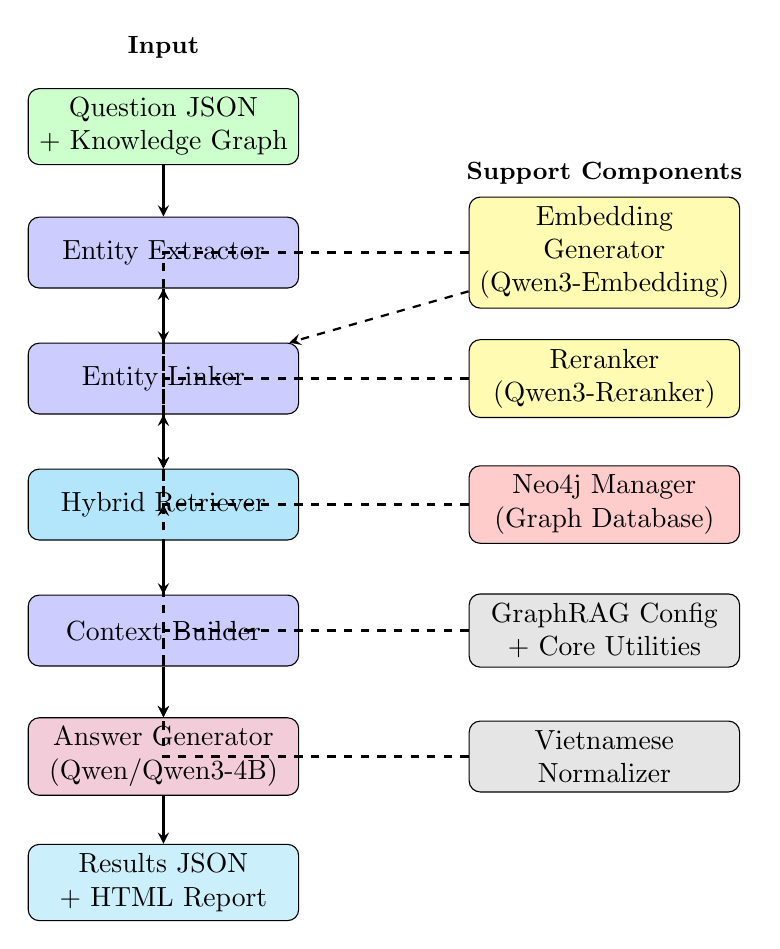
\begin{tikzpicture}[node distance=1.6cm, auto]
    % Styles
    \tikzstyle{datablock} = [rectangle, draw, fill=green!20, 
        text width=3.2cm, text centered, rounded corners, minimum height=0.9cm]
    \tikzstyle{component} = [rectangle, draw, fill=blue!20, 
        text width=3.2cm, text centered, rounded corners, minimum height=0.9cm]
    \tikzstyle{apiblock} = [rectangle, draw, fill=orange!20, 
        text width=3.2cm, text centered, rounded corners, minimum height=0.9cm]
    \tikzstyle{dbblock} = [rectangle, draw, fill=red!20, 
        text width=3.2cm, text centered, rounded corners, minimum height=0.9cm]
    \tikzstyle{modelblock} = [rectangle, draw, fill=purple!20, 
        text width=3.2cm, text centered, rounded corners, minimum height=0.9cm]
    \tikzstyle{outputblock} = [rectangle, draw, fill=cyan!20, 
        text width=3.2cm, text centered, rounded corners, minimum height=0.9cm]
    \tikzstyle{arrow} = [thick,->,>=stealth]
    \tikzstyle{dashedarrow} = [thick,->,>=stealth,dashed]
    
    % === LEFT COLUMN: Main Pipeline ===
    % Input
    \node [datablock] (input) {Question JSON\\+ Knowledge Graph};
    
    % Entity Extractor
    \node [component, below of=input] (entityext) {Entity Extractor};
    
    % Entity Linker
    \node [component, below of=entityext] (entitylink) {Entity Linker};
    
    % Hybrid Retriever
    \node [component, below of=entitylink, fill=cyan!30] (retriever) {Hybrid Retriever};
    
    % Context Builder
    \node [component, below of=retriever] (ctxbuilder) {Context Builder};
    
    % Answer Generator
    \node [modelblock, below of=ctxbuilder] (answergen) {Answer Generator\\(Qwen/Qwen3-4B)};
    
    % Output
    \node [outputblock, below of=answergen] (output) {Results JSON\\+ HTML Report};
    
    % === RIGHT COLUMN: Components ===
    % Embedding Generator
    \node [component, right of=entityext, xshift=4cm, fill=yellow!30] (embedding) {Embedding Generator\\(Qwen3-Embedding)};
    
    % Reranker
    \node [component, below of=embedding, fill=yellow!30] (reranker) {Reranker\\(Qwen3-Reranker)};
    
    % Neo4j Manager
    \node [dbblock, below of=reranker] (neo4j) {Neo4j Manager\\(Graph Database)};
    
    % Core/Config
    \node [datablock, below of=neo4j, fill=gray!20] (config) {GraphRAG Config\\+ Core Utilities};
    
    % Vietnamese Normalizer
    \node [datablock, below of=config, fill=gray!20] (normalizer) {Vietnamese\\Normalizer};
    
    % === ARROWS: Main Flow ===
    \draw [arrow] (input) -- (entityext);
    \draw [arrow] (entityext) -- (entitylink);
    \draw [arrow] (entitylink) -- (retriever);
    \draw [arrow] (retriever) -- (ctxbuilder);
    \draw [arrow] (ctxbuilder) -- (answergen);
    \draw [arrow] (answergen) -- (output);
    
    % === ARROWS: Dependencies ===
    \draw [dashedarrow] (embedding) -- (entitylink);
    \draw [dashedarrow] (embedding) -| (retriever);
    \draw [dashedarrow] (reranker) -| (retriever);
    \draw [dashedarrow] (neo4j) -| (retriever);
    \draw [dashedarrow] (neo4j) -| (entitylink);
    \draw [dashedarrow] (config) -| (answergen);
    \draw [dashedarrow] (normalizer) -| (entityext);
    
    % === Labels ===
    \node [above of=input, yshift=-0.6cm, font=\small\bfseries] {Input};
    \node [above of=embedding, yshift=-0.6cm, font=\small\bfseries] {Support Components};
    
\end{tikzpicture}
\caption{Kiến trúc tổng quan hệ thống GraphRAG QA Pipeline}
\label{fig:graphrag-qa-architecture}
\end{figure}


\begin{figure}[H]
\centering
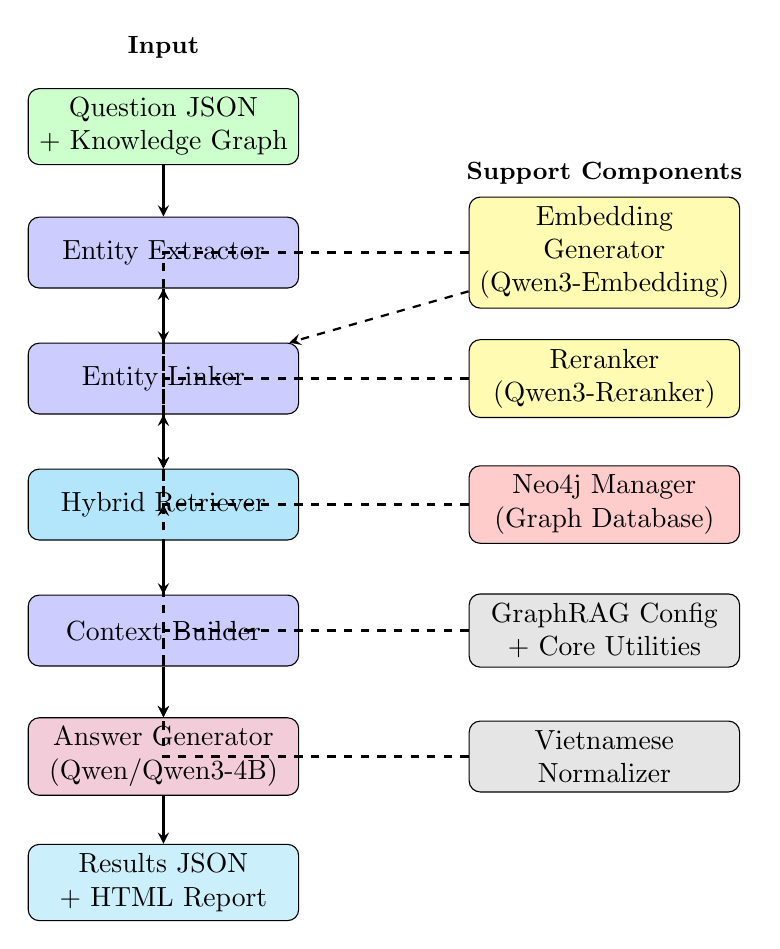
\begin{tikzpicture}[node distance=1.6cm, auto]
    % Styles
    \tikzstyle{datablock} = [rectangle, draw, fill=green!20, 
        text width=3.2cm, text centered, rounded corners, minimum height=0.9cm]
    \tikzstyle{component} = [rectangle, draw, fill=blue!20, 
        text width=3.2cm, text centered, rounded corners, minimum height=0.9cm]
    \tikzstyle{apiblock} = [rectangle, draw, fill=orange!20, 
        text width=3.2cm, text centered, rounded corners, minimum height=0.9cm]
    \tikzstyle{dbblock} = [rectangle, draw, fill=red!20, 
        text width=3.2cm, text centered, rounded corners, minimum height=0.9cm]
    \tikzstyle{modelblock} = [rectangle, draw, fill=purple!20, 
        text width=3.2cm, text centered, rounded corners, minimum height=0.9cm]
    \tikzstyle{outputblock} = [rectangle, draw, fill=cyan!20, 
        text width=3.2cm, text centered, rounded corners, minimum height=0.9cm]
    \tikzstyle{arrow} = [thick,->,>=stealth]
    \tikzstyle{dashedarrow} = [thick,->,>=stealth,dashed]
    
    % === LEFT COLUMN: Main Pipeline ===
    % Input
    \node [datablock] (input) {Question JSON\\+ Knowledge Graph};
    
    % Entity Extractor
    \node [component, below of=input] (entityext) {Entity Extractor};
    
    % Entity Linker
    \node [component, below of=entityext] (entitylink) {Entity Linker};
    
    % Hybrid Retriever
    \node [component, below of=entitylink, fill=cyan!30] (retriever) {Hybrid Retriever};
    
    % Context Builder
    \node [component, below of=retriever] (ctxbuilder) {Context Builder};
    
    % Answer Generator
    \node [modelblock, below of=ctxbuilder] (answergen) {Answer Generator\\(Qwen/Qwen3-4B)};
    
    % Output
    \node [outputblock, below of=answergen] (output) {Results JSON\\+ HTML Report};
    
    % === RIGHT COLUMN: Components ===
    % Embedding Generator
    \node [component, right of=entityext, xshift=4cm, fill=yellow!30] (embedding) {Embedding Generator\\(Qwen3-Embedding)};
    
    % Reranker
    \node [component, below of=embedding, fill=yellow!30] (reranker) {Reranker\\(Qwen3-Reranker)};
    
    % Neo4j Manager
    \node [dbblock, below of=reranker] (neo4j) {Neo4j Manager\\(Graph Database)};
    
    % Core/Config
    \node [datablock, below of=neo4j, fill=gray!20] (config) {GraphRAG Config\\+ Core Utilities};
    
    % Vietnamese Normalizer
    \node [datablock, below of=config, fill=gray!20] (normalizer) {Vietnamese\\Normalizer};
    
    % === ARROWS: Main Flow ===
    \draw [arrow] (input) -- (entityext);
    \draw [arrow] (entityext) -- (entitylink);
    \draw [arrow] (entitylink) -- (retriever);
    \draw [arrow] (retriever) -- (ctxbuilder);
    \draw [arrow] (ctxbuilder) -- (answergen);
    \draw [arrow] (answergen) -- (output);
    
    % === ARROWS: Dependencies ===
    \draw [dashedarrow] (embedding) -- (entitylink);
    \draw [dashedarrow] (embedding) -| (retriever);
    \draw [dashedarrow] (reranker) -| (retriever);
    \draw [dashedarrow] (neo4j) -| (retriever);
    \draw [dashedarrow] (neo4j) -| (entitylink);
    \draw [dashedarrow] (config) -| (answergen);
    \draw [dashedarrow] (normalizer) -| (entityext);
    
    % === Labels ===
    \node [above of=input, yshift=-0.6cm, font=\small\bfseries] {Input};
    \node [above of=embedding, yshift=-0.6cm, font=\small\bfseries] {Support Components};
    
\end{tikzpicture}
\caption{Kiến trúc tổng quan hệ thống GraphRAG QA Pipeline}
\label{fig:graphrag-qa-architecture}
\end{figure}


\begin{figure}[H]
\centering
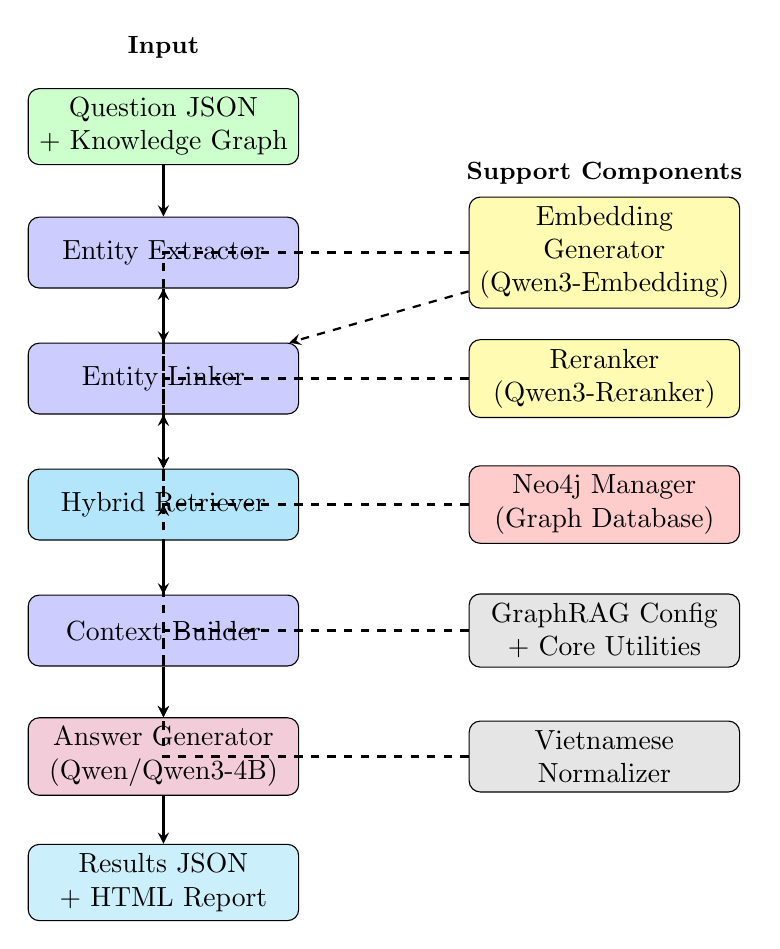
\begin{tikzpicture}[node distance=1.6cm, auto]
    % Styles
    \tikzstyle{datablock} = [rectangle, draw, fill=green!20, 
        text width=3.2cm, text centered, rounded corners, minimum height=0.9cm]
    \tikzstyle{component} = [rectangle, draw, fill=blue!20, 
        text width=3.2cm, text centered, rounded corners, minimum height=0.9cm]
    \tikzstyle{apiblock} = [rectangle, draw, fill=orange!20, 
        text width=3.2cm, text centered, rounded corners, minimum height=0.9cm]
    \tikzstyle{dbblock} = [rectangle, draw, fill=red!20, 
        text width=3.2cm, text centered, rounded corners, minimum height=0.9cm]
    \tikzstyle{modelblock} = [rectangle, draw, fill=purple!20, 
        text width=3.2cm, text centered, rounded corners, minimum height=0.9cm]
    \tikzstyle{outputblock} = [rectangle, draw, fill=cyan!20, 
        text width=3.2cm, text centered, rounded corners, minimum height=0.9cm]
    \tikzstyle{arrow} = [thick,->,>=stealth]
    \tikzstyle{dashedarrow} = [thick,->,>=stealth,dashed]
    
    % === LEFT COLUMN: Main Pipeline ===
    % Input
    \node [datablock] (input) {Question JSON\\+ Knowledge Graph};
    
    % Entity Extractor
    \node [component, below of=input] (entityext) {Entity Extractor};
    
    % Entity Linker
    \node [component, below of=entityext] (entitylink) {Entity Linker};
    
    % Hybrid Retriever
    \node [component, below of=entitylink, fill=cyan!30] (retriever) {Hybrid Retriever};
    
    % Context Builder
    \node [component, below of=retriever] (ctxbuilder) {Context Builder};
    
    % Answer Generator
    \node [modelblock, below of=ctxbuilder] (answergen) {Answer Generator\\(Qwen/Qwen3-4B)};
    
    % Output
    \node [outputblock, below of=answergen] (output) {Results JSON\\+ HTML Report};
    
    % === RIGHT COLUMN: Components ===
    % Embedding Generator
    \node [component, right of=entityext, xshift=4cm, fill=yellow!30] (embedding) {Embedding Generator\\(Qwen3-Embedding)};
    
    % Reranker
    \node [component, below of=embedding, fill=yellow!30] (reranker) {Reranker\\(Qwen3-Reranker)};
    
    % Neo4j Manager
    \node [dbblock, below of=reranker] (neo4j) {Neo4j Manager\\(Graph Database)};
    
    % Core/Config
    \node [datablock, below of=neo4j, fill=gray!20] (config) {GraphRAG Config\\+ Core Utilities};
    
    % Vietnamese Normalizer
    \node [datablock, below of=config, fill=gray!20] (normalizer) {Vietnamese\\Normalizer};
    
    % === ARROWS: Main Flow ===
    \draw [arrow] (input) -- (entityext);
    \draw [arrow] (entityext) -- (entitylink);
    \draw [arrow] (entitylink) -- (retriever);
    \draw [arrow] (retriever) -- (ctxbuilder);
    \draw [arrow] (ctxbuilder) -- (answergen);
    \draw [arrow] (answergen) -- (output);
    
    % === ARROWS: Dependencies ===
    \draw [dashedarrow] (embedding) -- (entitylink);
    \draw [dashedarrow] (embedding) -| (retriever);
    \draw [dashedarrow] (reranker) -| (retriever);
    \draw [dashedarrow] (neo4j) -| (retriever);
    \draw [dashedarrow] (neo4j) -| (entitylink);
    \draw [dashedarrow] (config) -| (answergen);
    \draw [dashedarrow] (normalizer) -| (entityext);
    
    % === Labels ===
    \node [above of=input, yshift=-0.6cm, font=\small\bfseries] {Input};
    \node [above of=embedding, yshift=-0.6cm, font=\small\bfseries] {Support Components};
    
\end{tikzpicture}
\caption{Kiến trúc tổng quan hệ thống GraphRAG QA Pipeline}
\label{fig:graphrag-qa-architecture}
\end{figure}
